{
Vi får at vide, at binomialfordelingen tilnærmer sig normalfordelingen
for store værdier af $n$. Dette ses i figur \ref{hist8_20_100}. For
$n = 8$ ses det at de observerede værdier fra simulationen ikke følger
normalfordelingen. Ved $n = 20$ ligger vi tættere på normalfordelingen.
For $n = 100$ ligger observationerne stort set på niveau med
normalfordelingen, men vi lægger også her mærke til at der i intervallet
$[24,26)$ er et højt antal observationer, som vi så i opgave 2. Også
intervallet $[30,32)$ ligger udenfor normalfordelingen, men her er der et
færre antal observationer.

\begin{figure}[!h]
    \centering
    \subfloat[$n = 8$ og $p = 0.25$]{
        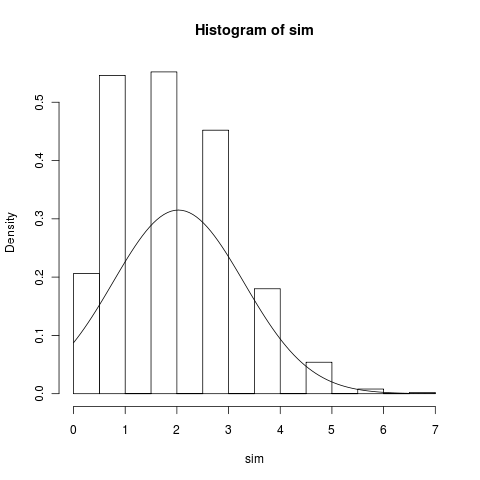
\includegraphics[width=0.5\textwidth]{8_hist_5}
        \label{hist_8}
    }
    \subfloat[$n = 20$ og $p = 0.25$]
        {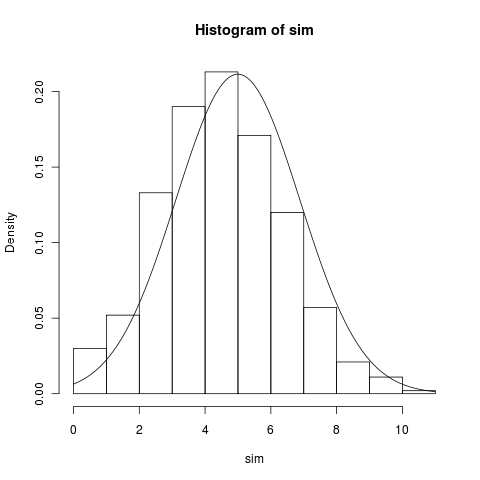
\includegraphics[width=0.5\textwidth]{20_hist_5}
        \label{hist_20}
    }\\
    \subfloat[$n = 100$ og $p = 0.25$]{
        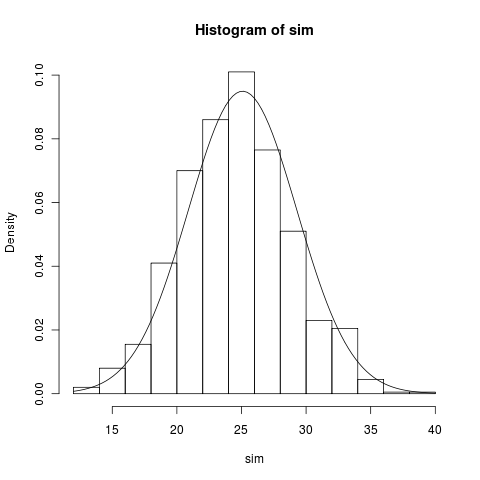
\includegraphics[width=0.5\textwidth]{100_hist_5}
        \label{hist_100}
    }
    \caption{Histogram og normalfordeling}
    \label{hist8_20_100}
\end{figure}

}
